\documentclass{article}
\usepackage[utf8]{inputenc}
\usepackage{amsmath}
\usepackage{graphicx}
\usepackage{hyperref}
\graphicspath{ {c:/Fanny/Documents/} }

\title{Time series analysis lab 1}
\author{Fanny Karelius (fanka300)}
\date{\today}

\begin{document}
\maketitle

\begin{section}{Analysis and results}
\begin{subsection}{Assignment 1}
\begin{figure}[ht!]
    \centering
    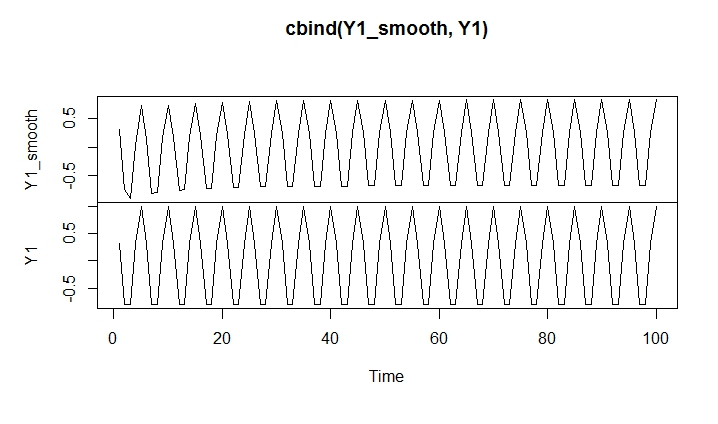
\includegraphics[scale=0.4]{cbindY1}
    \caption{Time series 1}
    \label{fig:ts1}
\end{figure}
\begin{figure}[ht!]
    \centering
    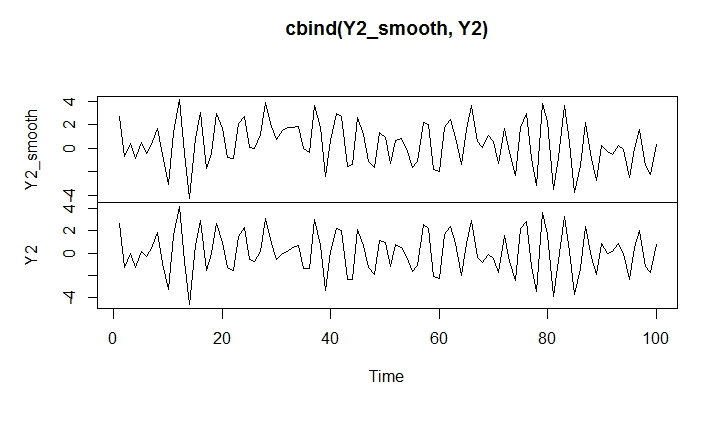
\includegraphics[scale=0.4]{cbindY2}
    \caption{Time series 2}
    \label{fig:ts2}
\end{figure}
\begin{figure}[ht!]
    \centering
    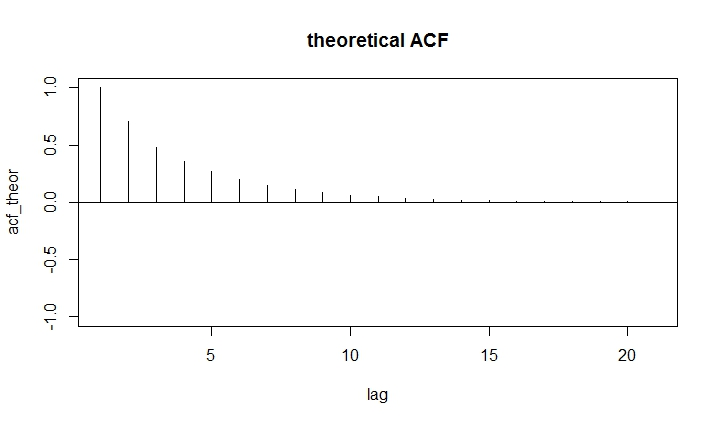
\includegraphics[scale=0.4]{acfTheo}
    \caption{Theoretical ACF}
    \label{fig:acf_theo}
\end{figure}
\begin{figure}[ht!]
    \centering
    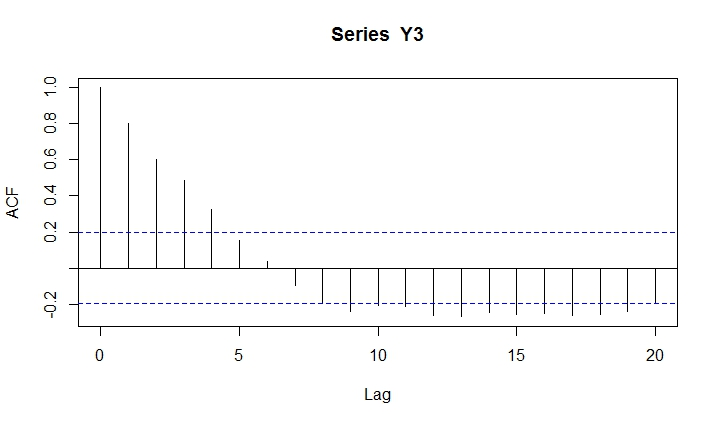
\includegraphics[scale=0.4]{acfY3}
    \caption{Sample ACF}
    \label{fig:acf_sample}
\end{figure}
\end{subsection}

\begin{subsection}{Assignment 2}
\begin{figure}[ht!]
    \centering
    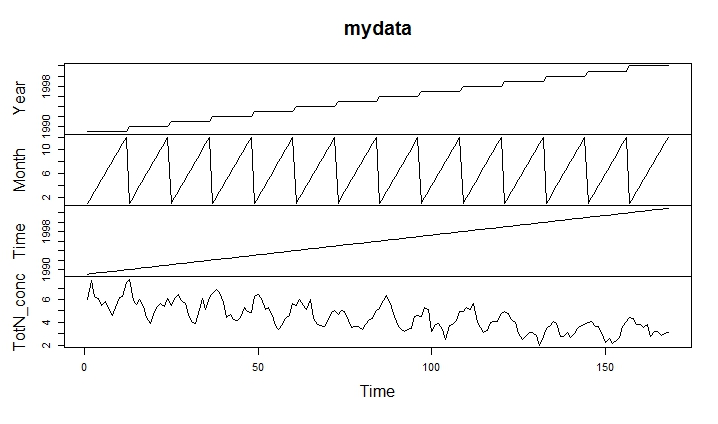
\includegraphics[scale=0.4]{mydata}
    \caption{Rhine river data}
    \label{fig:mydata}
\end{figure}
\begin{figure}[ht!]
    \centering
    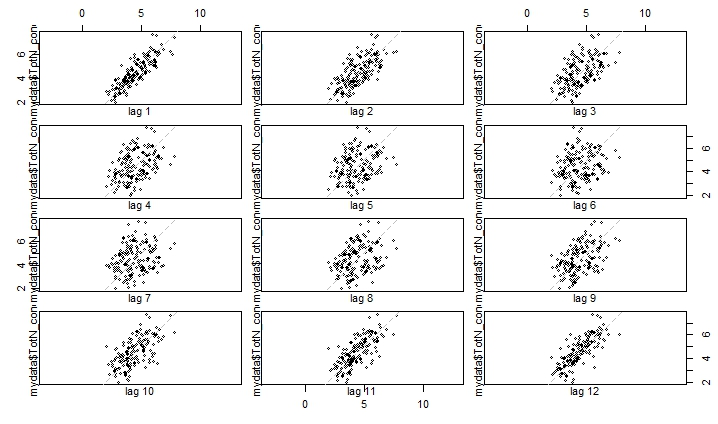
\includegraphics[scale=0.4]{mydata_scatter}
    \caption{Rhine river scatter plots}
    \label{fig:mydata_scatter}
\end{figure}
\begin{figure}[ht!]
    \centering
    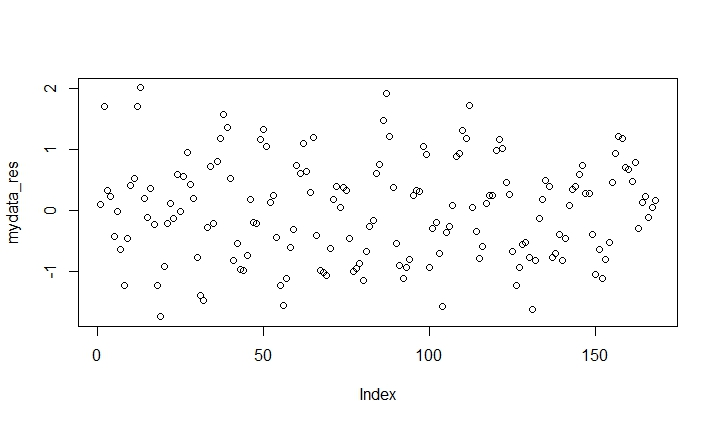
\includegraphics[scale=0.4]{mydata_res}
    \caption{Rhine river residuals}
    \label{fig:mydata_res}
\end{figure}
\begin{figure}[ht!]
    \centering
    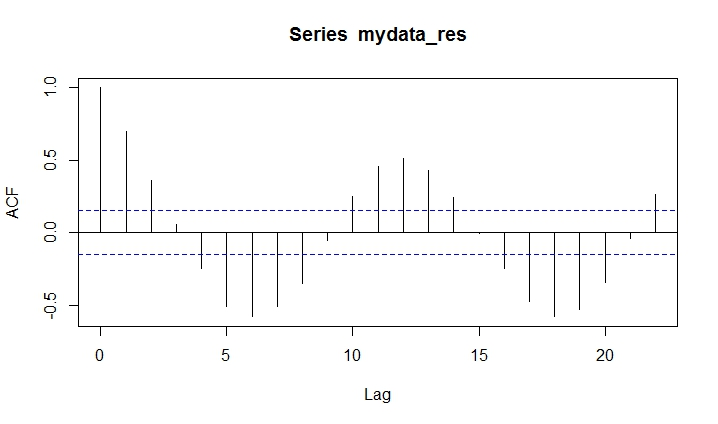
\includegraphics[scale=0.4]{mydata_resACF}
    \caption{ACF of residuals}
    \label{fig:mydata_resACF}
\end{figure}
\begin{figure}[ht!]
    \centering
    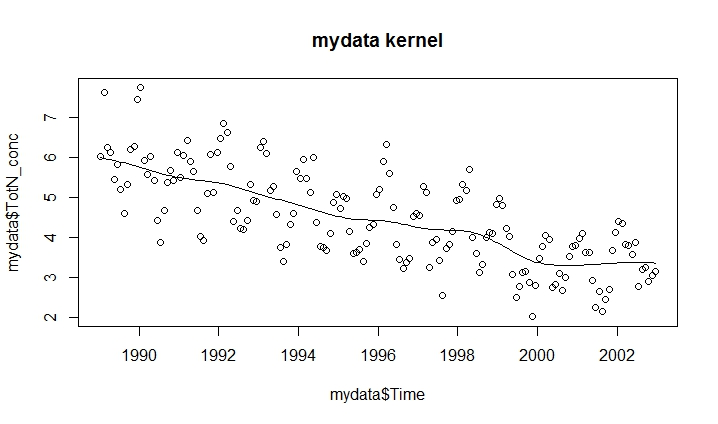
\includegraphics[scale=0.4]{mydata_kernel}
    \caption{Kernel smoother}
    \label{fig:mydata_kernel}
\end{figure}
\begin{figure}[ht!]
    \centering
    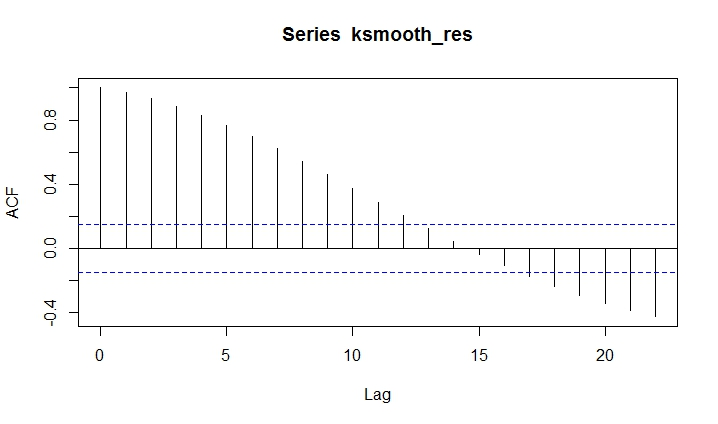
\includegraphics[scale=0.4]{ksmooth_res}
    \caption{Kernel smoother ACF}
    \label{fig:ksmooth_acf}
\end{figure}
\begin{figure}[ht!]
    \centering
    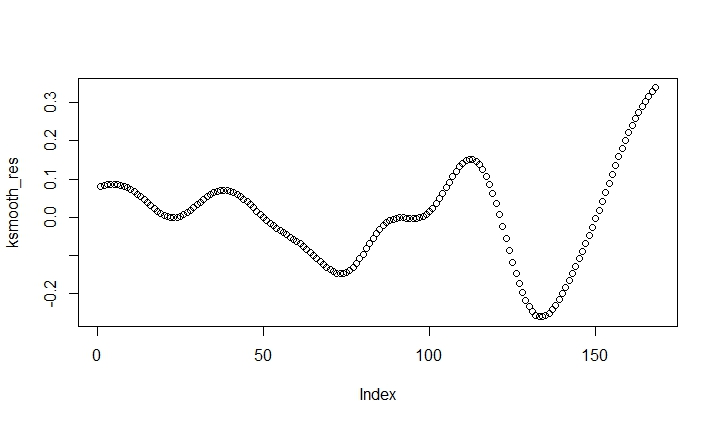
\includegraphics[scale=0.4]{ksmoothRES}
    \caption{Kernel smoother residuals}
    \label{fig:ksmooth_res}
\end{figure}
\begin{figure}[ht!]
    \centering
    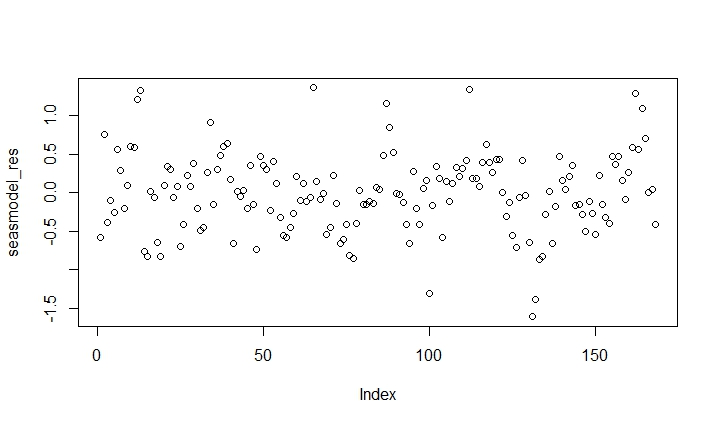
\includegraphics[scale=0.4]{seasmodel_res1}
    \caption{Seasonal means model residuals}
    \label{fig:seasmodel_res}
\end{figure}
\begin{figure}[ht!]
    \centering
    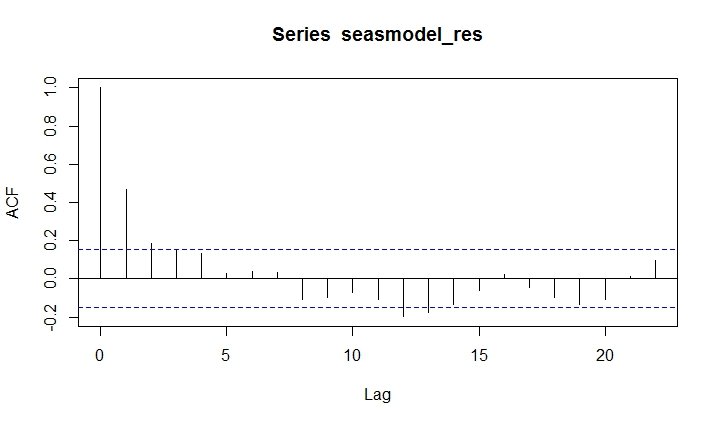
\includegraphics[scale=0.4]{seasmodel_res}
    \caption{Seasonal means model ACF}
    \label{fig:seasmodel_acf}
\end{figure}
\end{subsection}

\begin{subsection}{Assignment 3}
\begin{figure}[ht!]
    \centering
    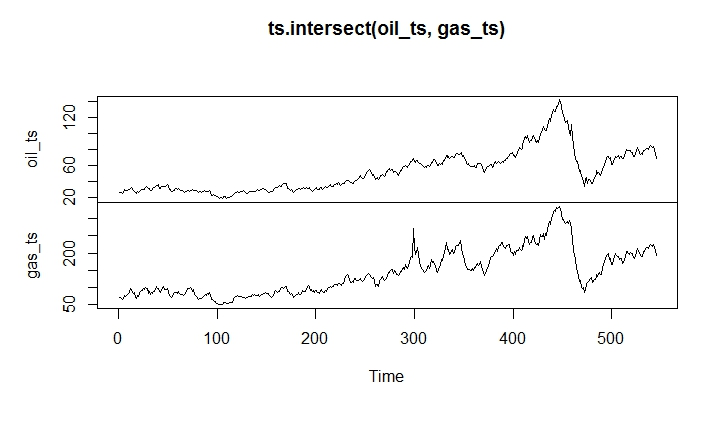
\includegraphics[scale=0.4]{oilandgas}
    \caption{Oil and gas prices}
    \label{fig:oilandgas}
\end{figure}
\begin{figure}[ht!]
    \centering
    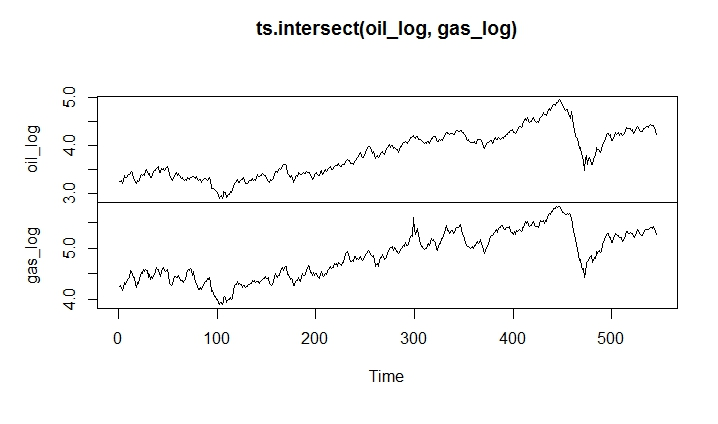
\includegraphics[scale=0.4]{oilandgaslog}
    \caption{Log transform of oil and gas prices}
    \label{fig:oilandgaslog}
\end{figure}
\begin{figure}[ht!]
    \centering
    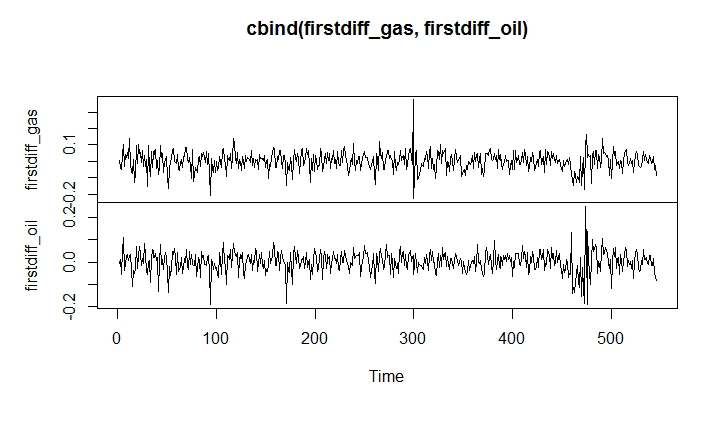
\includegraphics[scale=0.4]{oilandgasfirstdiff}
    \caption{First difference}
    \label{fig:oilandgasfirstdiff}
\end{figure}
\begin{figure}[ht!]
    \centering
    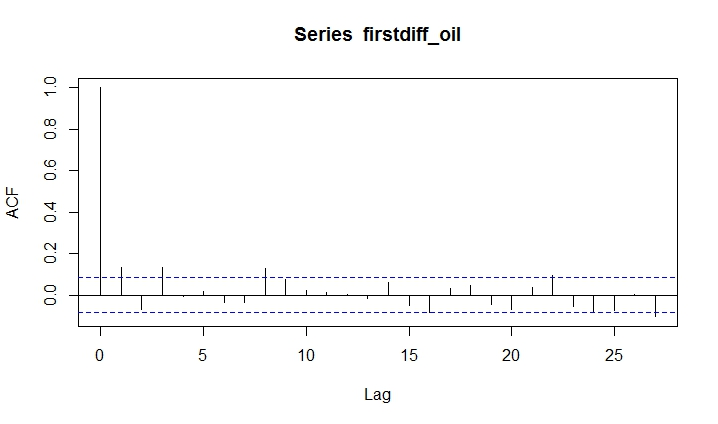
\includegraphics[scale=0.4]{oilfirstdiff_res}
    \caption{ACF first difference oil}
    \label{fig:oil_acf}
\end{figure}
\begin{figure}[ht!]
    \centering
    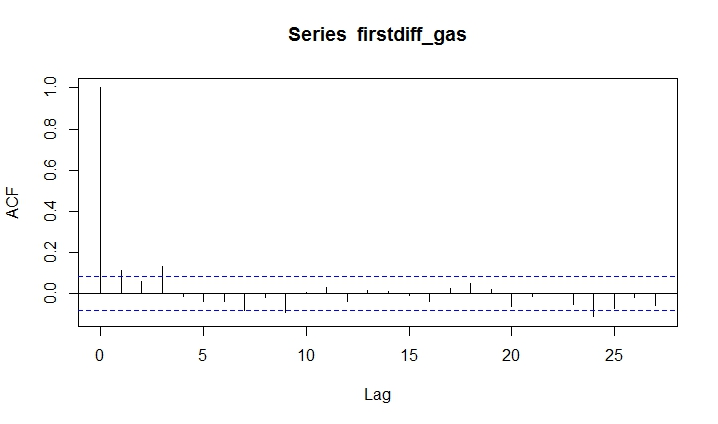
\includegraphics[scale=0.4]{gasfirstdiff_res}
    \caption{ACF first difference gas}
    \label{fig:gas_acf}
\end{figure}
\begin{figure}[ht!]
    \centering
    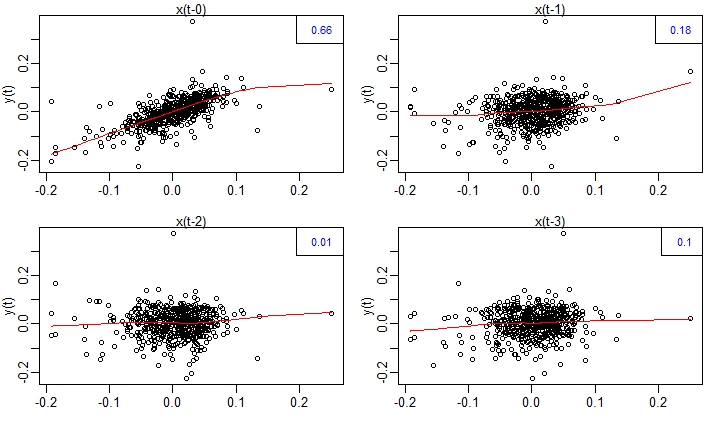
\includegraphics[scale=0.4]{oilandgaslag}
    \caption{Scatter plots for oil and gas}
    \label{fig:oilandgas_scatter}
\end{figure}
\begin{figure}[ht!]
    \centering
    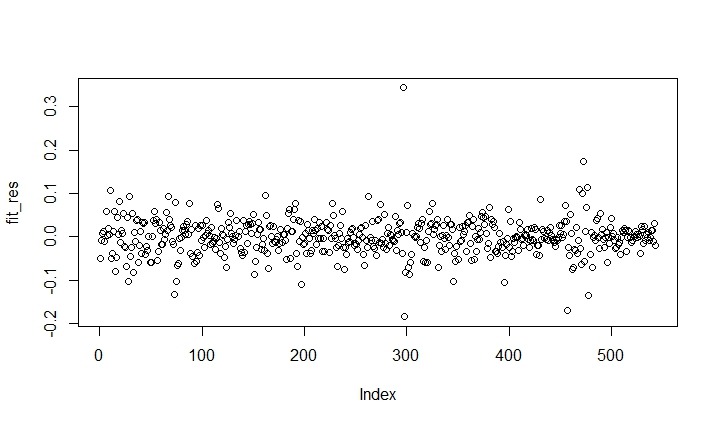
\includegraphics[scale=0.4]{fitmodel_res}
    \caption{Residuals for fitted model}
    \label{fig:fitmodel_res}
\end{figure}
\begin{figure}[ht!]
    \centering
    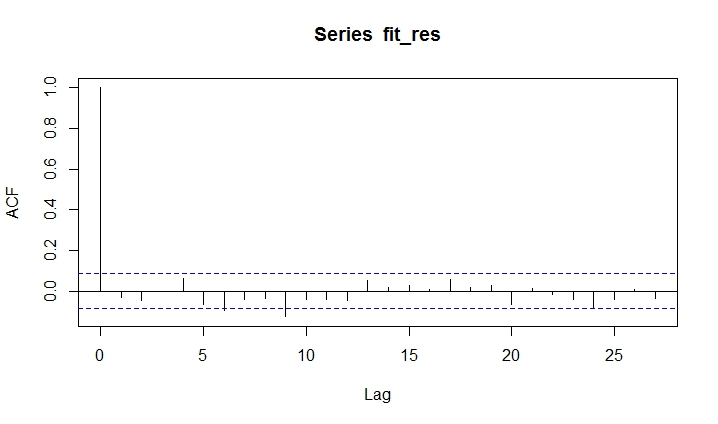
\includegraphics[scale=0.4]{fitmodel_acf}
    \caption{ACF for fitted model}
    \label{fig:fitmodel_acf}
\end{figure}
\end{subsection}


\end{section}
\pagebreak
\begin{section}{Appendix}
\begin{verbatim}

#ASSIGNMENT 1

#a)

  #Time series 1: y(t)=cos(2*pi*t/5)
t<-seq(1,100, by=1)
Y1<-cos(2*pi*t/5)
plot(t,Y1, type="o", main="TS 1")
grid()
Y1_smooth<- filter(Y1, 0.2*c(1,1,1,1), method="recursive")
plot(t,Y1_smooth, type="o", main="Smooth TS 1")
grid()
plot(cbind(Y1_smooth, Y1))
  #Time series 2: y(t)=-0.8*x(t-2)+w(t)
set.seed(12345)
Y2 <- arima.sim(model=list(ar=c(0,-0.8)),n=100)
plot(Y2, type="o", main="TS 2")
grid()
Y2_smooth<- filter(Y2, 0.2*c(1,1,1,1), method="recursive")
plot(t,Y2_smooth, type="o", main="Smooth TS 2")
grid()
plot(cbind(Y2_smooth, Y2))

#b)
z_causal<- c(1,-4,2,0,0,1)
polyroot(z_causal)
#some roots outside unit circle, but not all so not causal

z_inv <- c(1,0,3,0,1,0,-4)
polyroot(z_inv)
#some roots outside unit circle, but not all so not invertible

#c) x(t)+0.75x(t-1)=w(t)-w(t-2)/9
set.seed(54321)
Y3<-arima.sim(list(order=c(1,0,2), ar=0.75, ma=c(0,-(1/9))), n=100)
acf_sample <- acf(Y3)
acf_theor <- ARMAacf(ar=0.75, ma=c(0,-(1/9)),pacf = FALSE,lag.max = 20)
plot(acf_theor, type="h", xlab="lag", ylim=c(-1,1)); abline(h=0)
acf_sample[1:3]
acf_theor

#ASSIGNMENT 2

#a)
mydata <- read.csv(file="Rhine1.csv", sep=";")
plot.ts(mydata, main="mydata")
pairs(mydata)
lag.plot(mydata$TotN_conc,lags = 12)

#b)
mydata_fit <- lm(mydata$TotN_conc~mydata$Time,data=mydata, na.action = na.omit)
mydata_fit
summary(mydata_fit)
mydata_res<- residuals(mydata_fit)
plot(mydata_res)
acf(mydata_res)

#c)
mydata_ksmooth <- ksmooth(x=mydata$Time, y=mydata$TotN_conc,"normal", bandwidth = 2)
plot(x = mydata$Time, y= mydata$TotN_conc, main="mydata kernel")
lines(mydata_ksmooth)
ksmooth_reg<- lm(mydata_ksmooth$y~mydata_ksmooth$x, data=mydata_ksmooth, na.action=na.omit)
summary(ksmooth_reg)
ksmooth_res <- residuals(ksmooth_reg)
acf(ksmooth_res)
plot(ksmooth_res)

#d)
Month1 <- ifelse(mydata$Month==1,1,0)
Month2 <- ifelse(mydata$Month==2,1,0)
Month3 <- ifelse(mydata$Month==3,1,0)
Month4 <- ifelse(mydata$Month==4,1,0)
Month5 <- ifelse(mydata$Month==5,1,0)
Month6 <- ifelse(mydata$Month==6,1,0)
Month7 <- ifelse(mydata$Month==7,1,0)
Month8 <- ifelse(mydata$Month==8,1,0)
Month9 <- ifelse(mydata$Month==9,1,0)
Month10 <- ifelse(mydata$Month==10,1,0)
Month11 <- ifelse(mydata$Month==11,1,0)
Month12 <- ifelse(mydata$Month==12,1,0)
seas_model <- lm(mydata$TotN_conc~mydata$Time+Month1+Month2+Month3+Month4+
Month5+Month6+Month7+Month8+Month9+Month10+Month11+Month12)
summary(seas_model)
seasmodel_res <- residuals(seas_model)
acf(seasmodel_res)
plot(seasmodel_res)

#e)
seas_step<-step(seas_model)
seas_step
seas_step$anova

#ASSIGNMENT 3

#a) install package astsa, library(astsa)
library(astsa)
oil_ts <- ts(oil)
gas_ts <- ts(gas)
plot(ts.intersect(oil_ts,gas_ts))

#b) log transformation
oil_log <- log(oil_ts)
gas_log <- log(gas_ts)
plot(ts.intersect(oil_log, gas_log))

#c) detrended, first difference, x_t = oil, y_t = gas
firstdiff_oil <- diff(oil_log)
plot(firstdiff_oil, main="First difference oil_log")
firstdiff_gas <- diff(gas_log)
plot(firstdiff_gas, main ="First difference gas_log")
plot(cbind(firstdiff_gas,firstdiff_oil))
acf(firstdiff_gas)
acf(firstdiff_oil)
oil_log_reg <- lm(oil_log~time(oil_log), na.action=NULL)
oil_log_res <- residuals(oil_log_reg)
gas_log_reg <- lm(gas_log~time(gas_log), na.action=NULL)
gas_log_res <- residuals(gas_log_reg)

plot(cbind(oil_log_res,gas_log_res))
x<- firstdiff_oil
y<- firstdiff_gas

#d)
lag2.plot(series1 = x, series2 = y, max.lag = 3)

#e)
indi <- ifelse(x<0,0,1)
mess <- ts.intersect(y, x, x2=lag(x,-1), indi)
summary(fit <- lm(y~ x + x2 + indi, data=mess))
fit_res<-residuals(fit)
plot(fit_res)
acf(fit_res)

\end{verbatim}
\end{section}

\end{document}
